%
% Documento: Ilustração
%

\chapter{ILUSTRAÇÕES}

A apresentação de quadros e tabelas está regida pelas Normas de Apresentação Tabular do Instituto Brasileiro de Geografia e Estatística.

\section{Figuras}

São desenhos, fotografias, organogramas, esquemas etc. com os respectivos títulos pre-cedidos da palavra Figura e do número de ordem em algarismo arábico.

\begin{figure}[H]
    \centering
    \caption{Exemplo de figura}
    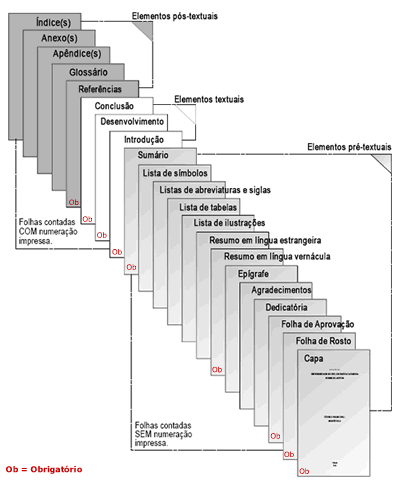
\includegraphics[width=0.5\textwidth]{figuras/abnt}
    \label{fig:ilustfig}
    {\fonte{Disponível em: <https://www.gazetadopovo.com.br/abntemfoco>. Acesso em: 24 de jan. de 2015.}}
\end{figure}

Os títulos devem ser colocados acima das figuras. No texto devem
ser indicados pela pa-lavra Figura acompanhada do número de ordem. E abaixo deve ser indicada sua fonte.

\section{Tabelas}

Tabelas são conjuntos de dados numéricos, associados a um
fenômeno, dispostos numa determinada ordem da classificação. Expressam as variações qualitativas e quantitativas de um fenômeno. A finalidade básica da tabela é resumir ou sintetizar dados de maneira a fornecer o máximo de informações num mínimo de espaço.

Na apresentação de uma tabela devem ser levados em consideração
os alguns critérios. Toda tabela deve ter significado próprio, dispensando consultas ao texto. A tabela deve ser colo-cada em posição vertical, para facilitar a leitura dos dados. No caso em que isso seja impossível, deve ser colocada em posição horizontal, com o título voltado para a margem esquerda da folha.

Se a tabela ou quadro não couber em uma página, deve ser
continuado na página seguin-te. Neste caso o final não será delimitado por traço horizontal na parte inferior e o cabeçalho será repetido na página seguinte. No texto devem ser indicadas pela palavra Tabela acompanha-da do número de ordem em algarismo arábico.

\begin{table}[htb]
	\IBGEtab{%
		\caption{Um Exemplo de tabela alinhada que pode ser longa
			ou curta, conforme padrão IBGE.}%
		\label{tabela-ibge}
	}{%
		\begin{tabular}{ccc}
			\toprule
			Nome & Nascimento & Documento \\
			\midrule \midrule
			Maria da Silva & 11/11/1111 & 111.111.111-11 \\
			\midrule 
			João Souza & 11/11/2111 & 211.111.111-11 \\
			\midrule 
			Laura Vicuña & 05/04/1891 & 3111.111.111-11 \\
			\bottomrule
		\end{tabular}%
	}{%
		\fonte{Produzido pelos autores.}%
		\nota{Esta é uma nota, que diz que os dados são baseados na
			regressão linear.}%
		\nota[Anotações]{Uma anotação adicional, que pode ser seguida de várias
			outras.}%
	}
\end{table}

\section{Gráficos}

Depois de sintetizados em tabelas, os dados podem ser
apresentados em gráficos, com a fi-nalidade de proporcionar ao interessado uma visão rápida do comportamento do fenômeno. Serve para representar qualquer tabela de maneira simples, legível e interessante, tornando cla-ros os fatos que poderiam passar despercebidos em dados apenas tabulados.

O elemento de identificação ordenado do gráfico, ou seja, o
número de ordem do mesmo no trabalho. No texto devem ser indicados pela palavra Gráfico, acompanhada do número de ordem em algarismo arábico.